\documentclass[a4paper, 10pt]{article}

\usepackage{algorithm}
\usepackage{algorithmic}
\usepackage{minted}
\usepackage{graphicx}
\usepackage{tabularx}
\usepackage{syntax}
\usepackage{fullpage}
\usepackage{amsmath}
\DeclareMathOperator*{\argmin}{argmin}
\DeclareMathOperator*{\argmax}{argmax}
%\usepackage{amsfonts}
\usepackage{stix}
\usepackage{hyperref}
\usepackage{tikz}
%\usetikzlibrary{graphs}
%\usepackage{libertine}
%\usepackage[T1]{fontenc}

\title{Channel Allocation in SC-FDMA: research assignment}
\author{Noric Couderc}
\date{\today}

\begin{document}

\maketitle
\tableofcontents

\section{Current progress}

\subsection*{Model}

Before introducing the model, we introduce a notation that will be used in this document.
\begin{itemize}
    \item Values are denoted in lowercase letters: $m, n$.
    \item Sets are denoted in uppercase letters: $N$.
    \item Some numerical sets are denoted in bold: like $\mathbb{N}$ or $\mathbb{R}$.
    \item Set families are denoted in calligraphic script: $\mathscr{F} = \{ N | N \subseteq \mathbb{N}\}$.
\end{itemize}

Here is presented a slightly different formulation of the model of the \textbf{Max-Utility} problem. 
When a function is not defined here, it is provided as a parameter.

\begin{itemize}
    \item Set of users: $M = \{1,\dots,m\}, m \in \mathbb{N}$.
    \item Set of channels: $N = \{1,\dots,n\}, n \in \mathbb{N}$.
    \item Set of all possible blocks: 
        $\mathscr{B} := \{ B_i | i \in M, B_i \subseteq N \}$.
    \item Power limit function of a user: $p_u : M \rightarrow \mathbb{R}^+$.
    \item Channels peak power limit of a channel: $p_s : N \rightarrow \mathbb{R}^+$.
    \item Power function of user $u$ on channel $c$,
        given $u$ has $n$ allocated channels:\\
        $p : (M \times N \times \mathbb{N}) \rightarrow \mathbb{R}^+$,
        with $p(u, c, n) = \min\{\frac{p_u(u)}{n}, p_s(c)\}$.
    \item Power function for an allocated block: 
        $p_B : (M \times \mathscr{B}) \rightarrow \mathbb{R}$, 
        with $p_B(u, B) = \sum_{c \in B} p(u, c, |B|)$.
    \item Utility function: 
        $u : (M \times \mathscr{B}) \rightarrow \mathbb{R}$.
\end{itemize}

The \textbf{Max-Utility} problem is defined as finding a relation $A \subseteq \{ (i, B_i) | i \in M, B_i \in \mathscr{B} \}$, 
where $A$ satisfies several constraints:
\begin{itemize}
    \item All users are allocated a block: $\forall i \in M (\exists (i, B_i) \in A)$.
    \item $\forall (i, B_i) \in A (B_i \neq \emptyset)$.
    \item $\forall (i, j) \in (M \times M)~(i \neq j \rightarrow B_i \cap B_h = \emptyset)$
    \item $A$ maximizes the function: $\sum_{(i, B_i) \in A} u(i, B_i)$.
\end{itemize}

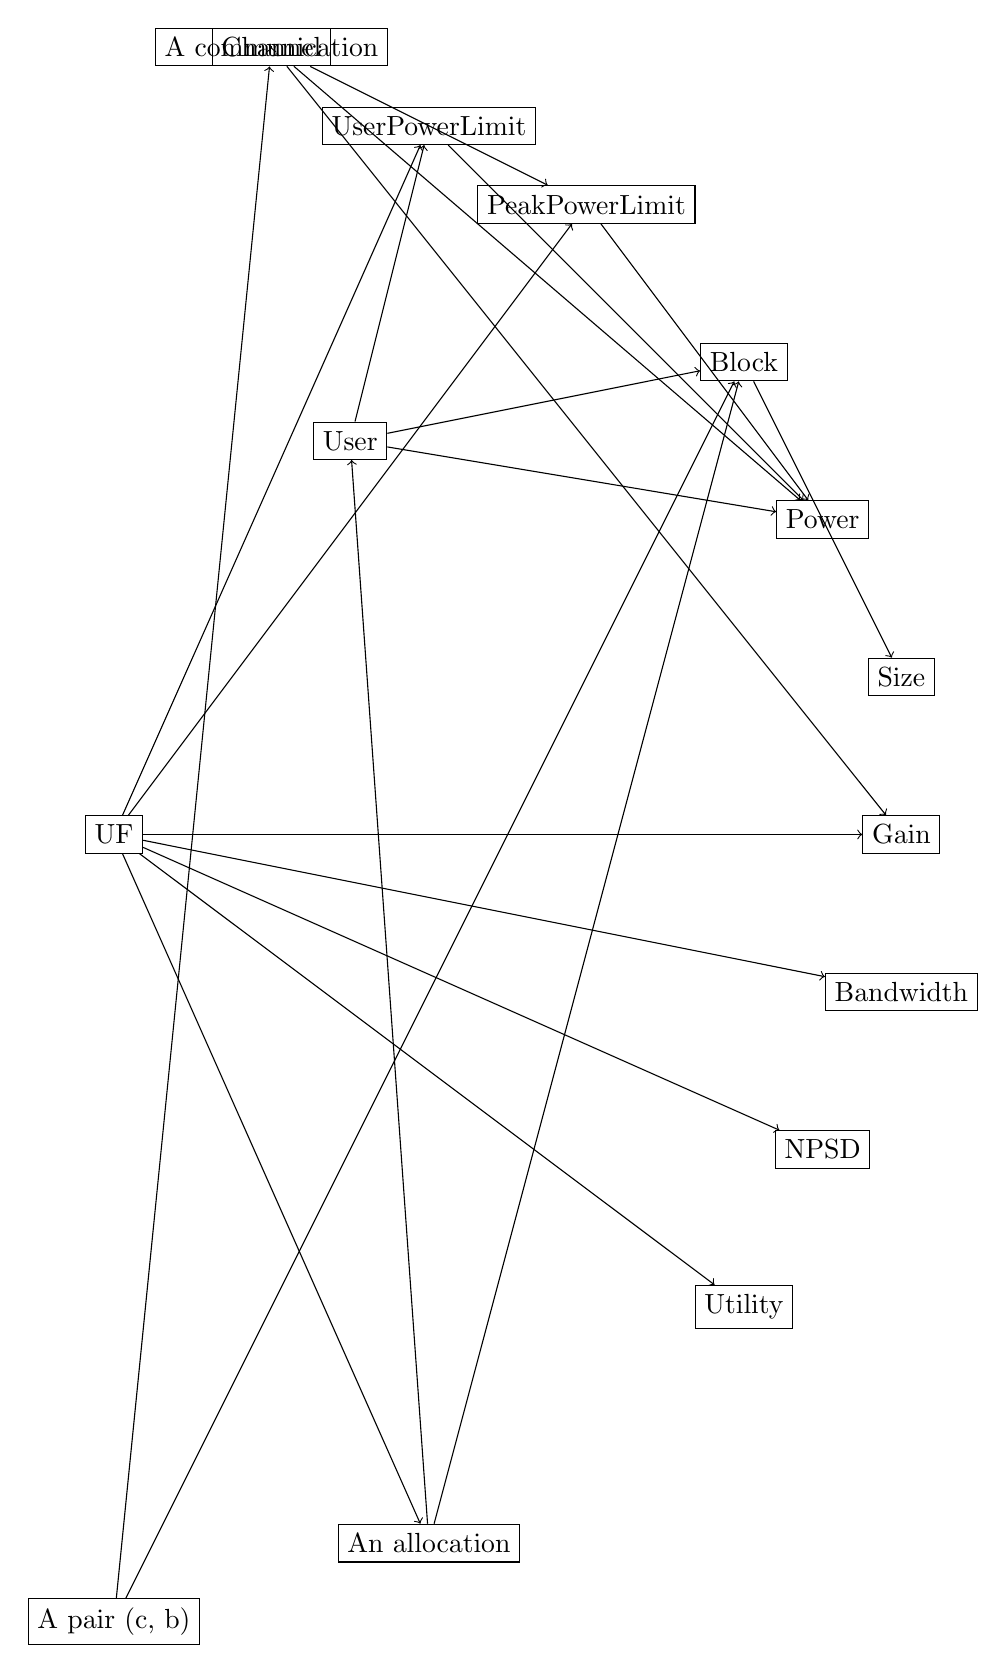
\begin{tikzpicture}
%[(0,10),(2,10),(4,9),(6,8),(8,6),(9,4),(10,2),(10,0),(10,-2),(9,-4),(8,-6),(6,-8),(4,-9),(2,-10),(0,-10),(-2,-10),(-4,-9),(-6,-8),(-8,-6),(-9,-4),(-10,-2),(-10,0),(-10,2),(-9,4),(-8,6),(-6,8),(-4,9),(-2,10),(0,10)]
    \node[draw] (User) at (3,5) {User};
    \node[draw] (Channel) at (2,10) {Channel};
    \node[draw] (UPL) at (4, 9) {UserPowerLimit};
    \node[draw] (PKPL) at (6, 8) {PeakPowerLimit};
    \node[draw] (Block) at (8, 6) {Block};
    \node[draw] (Power) at (9,4) {Power};
    \node[draw] (Size) at (10, 2) {Size};
    \node[draw] (Gain) at (10, 0) {Gain};
    \node[draw] (Bandwidth) at (10, -2) {Bandwidth};
    \node[draw] (NPSD) at (9, -4) {NPSD};
    \node[draw] (Utility) at (8,-6) {Utility};
    \node[draw] (UF) at (0, 0) {UF};
    \node[draw] (Alloc) at (4, -9) {An allocation};
    \node[draw] (Comm) at (2, 10) {A communication};
    \node[draw] (Pair) at (0, -10) {A pair (c, b)};

    \draw[->] (User) to (Power);
    \draw[->] (User) to (UPL);
    \draw[->] (User) to (Block);

    \draw[->] (Channel) to (PKPL);

    \draw[->] (UPL) to (Power);

    \draw[->] (PKPL) to (Power);

    \draw[->] (Block) to (Size);

    \draw[->] (UF) to (Gain);
    \draw[->] (UF) to (PKPL);
    \draw[->] (UF) to (UPL);
    \draw[->] (UF) to (Alloc);
    \draw[->] (UF) to (Bandwidth);
    \draw[->] (UF) to (Utility);
    \draw[->] (UF) to (NPSD);

    \draw[->] (Alloc) to (User);
    \draw[->] (Alloc) to (Block);

    \draw[->] (Comm) to (Channel);
    \draw[->] (Comm) to (Power);
    \draw[->] (Comm) to (Gain);

    \draw[->] (Pair) to (Channel);
    \draw[->] (Pair) to (Block);

\end{tikzpicture}


\subsection*{Algorithm}

\subsubsection*{Data structures}
\begin{itemize}
    \item A \textbf{Label} is a tuple of the form: $(v_\ell, m_\ell, M_\ell)$ 
        where $v_\ell$ is the performance value,
        $M_\ell$ is a subset of $M$, 
        and $m_\ell = |M_\ell|$.
    \item A \textbf{Bucket} is a list of labels. It stores a maximum of $k$ labels.
    \item A \textbf{Node} is a list of buckets. A node has $m + 1$ buckets, numbered as $0, 1, \dots, m$.
\end{itemize}

Labels are ordered according to a relation called a domination rule. 
We denote this order by defining the operator $\geq$ on labels:
\begin{align*}
    a \geq b \leftrightarrow v_a \geq v_b \land M_a \subseteq M_b
\end{align*}

\subsection*{Algorithm decomposition}

Here, the algorithm is divided in several components that have different purposes.
In this section $L(j,m)$ refers to the $m$th bucket in node $j$, therefore, $L$ is a list of nodes.

\begin{algorithm}
    \caption{Graph labeling algorithm}
    \label{alg:GLA algorithm}
    \begin{algorithmic}
        \STATE initialize $L$ using algorithm \ref{alg:initialization}.
        \FORALL{$j \in \{1, \dots, n\}$} 
            \FORALL{$m' \in \{1, \dots, \min(j, m)\}$}
                \FORALL{$i \in \{0, \dots, j-1\}$}
                    \STATE $L' \leftarrow L(i, m')$
                    \STATE allocate new users with algorithm \ref{alg:newusers}.
                    \STATE store labels in buckets with algorithm \ref{alg:insertlabels}.
                \ENDFOR
            \ENDFOR
        \ENDFOR
        \STATE $\ell^* \leftarrow \argmax_{\ell \in L(n,j), j = 1, \dots, m} v_\ell$
        \RETURN $\ell^*$
    \end{algorithmic}
\end{algorithm}

\begin{algorithm}
    \caption{Initialization}
    \label{alg:initialization}
    \begin{algorithmic}
        \REQUIRE $n$, $m$
        \FORALL{$j \in \{0, \dots, n\}$}
            \STATE $L(j, 0) \leftarrow \{ (0, 0, \emptyset) \}$
            \FORALL{$m' \in \{1, \dots, m\}$}
                \STATE $L(j, m') \leftarrow \emptyset$
            \ENDFOR
        \ENDFOR
    \RETURN $L$, a list of nodes
    \end{algorithmic}
\end{algorithm}

\begin{algorithm}
    \caption{Allocation of new users and creation of new labels}
    \label{alg:newusers}
    \begin{algorithmic}
        \REQUIRE $L$ a list of nodes, 
                 $L'$ a bucket,
                 $M$, 
                 $j \in N$,
                 $i \in \{0, \dots j - 1\}$,
                 $m \in M$,
                 $m' \in \{1, \dots \min(j, m)\}$,
                 $u : (M \times \mathscr{B}) \rightarrow \mathbb{R}$
        \FORALL{$\ell \in L(i, m'-1)$}
            \FORALL{$w \in M \setminus M_\ell$}
                \STATE $v_{i+1, j}^w \leftarrow u(w, \{i+2, \dots, j\})$
                \STATE $L' \leftarrow L' \cup \{(v_\ell + v_{i+1, j}^w, m_\ell + 1, M_\ell \cup \{w\})\}$
            \ENDFOR
        \ENDFOR
        \RETURN $L'$
    \end{algorithmic}
\end{algorithm}

\begin{algorithm}
    \caption{Insertion of labels in $L'$ in $L(j, m)$}
    \label{alg:insertlabels}
    \begin{algorithmic}
        \REQUIRE $L'$ a bucket,
                 $L$ a list of nodes,
                 $j \in N$,
                 $m \in M$
        \FORALL{$\ell'$ in $L'$}
            \IF{$\forall s \in \{1, \dots,  m\} (\nexists h \in L(j, s) (h \geq \ell'))$}
                \STATE insert $\ell'$ in $L(j, m)$ using algorithm \ref{alg:insertlabel}.
            \ENDIF
        \ENDFOR
    \end{algorithmic}
\end{algorithm}

\begin{algorithm}
    \caption{Insertion of a label $\ell'$ in $L(j,m)$} 
    \label{alg:insertlabel}
    \begin{algorithmic}
        \REQUIRE $L$ a list of nodes,
                 $\ell'$ a label,
                 $j \in N$,
                 $m \in M$,
                 $k \in \mathbb{N}$
        \IF{$|L(j, m)| \leq k$}
            \STATE $L(j, m) \leftarrow L(j, m) \cup \{ \ell' \}$
        \ELSE
            \STATE $\bar{\ell} \leftarrow \argmin_{h \in L(j, m)}v_h$
            \IF{$v_{\ell'} > v_{\bar{\ell}}$}
                \STATE $L(j,m) \leftarrow L(j,m) \setminus \{ \bar{\ell} \}$
                \STATE $L(j,m) \leftarrow L(j,m) \cup      \{ \ell' \}$
            \ENDIF
        \ENDIF
    \end{algorithmic}
\end{algorithm}

% \section{Plan}

% \subsection*{Risks}

% \section{Feedback}

\end{document}
